\documentclass[12pt,a4paper]{article}
\usepackage[utf8]{inputenc}
\usepackage[spanish]{babel}
\usepackage{graphicx}
\usepackage{listings}
\usepackage{hyperref}
\usepackage{geometry}
\usepackage{float}
\usepackage{caption}
\usepackage{tabularx}
\usepackage{booktabs}
\usepackage{tikz}
\usetikzlibrary{shapes.geometric, arrows.meta, positioning}

% Configuración de márgenes
\geometry{top=2.5cm, bottom=2.5cm, left=2.5cm, right=2.5cm}

% Configuración de la ruta de imágenes para Overleaf
% Busca imágenes tanto en la carpeta 'Entregable 2' como en la raíz './'
\graphicspath{{Entregable 2/}{./}}

% Estilo de enlaces
\hypersetup{
    colorlinks=true,
    linkcolor=blue,
    filecolor=magenta,      
    urlcolor=cyan,
    pdftitle={Trabajo Práctico Integrador -- ARQ-WEB 2026 (Entregables 1 y 2)},
}

\title{\textbf{Trabajo Práctico Integrador -- ARQ-WEB 2026}\\Despliegue, conectividad y verificación experimental de una aplicación web}
\author{Sofia Mereles \and Alba Martinez \and Guillermo Gonzalez}
\date{FP-UNA -- 2026}

\begin{document}

\maketitle

\begin{abstract}
El presente informe documenta la Fase 1 y Fase 2 del proyecto integrador de la asignatura Arquitectura Web. En la primera etapa se estableció la línea base de la infraestructura servidor mediante la configuración de un entorno virtualizado en Ubuntu Server en modo puente (\textit{Bridged}), evaluando y seleccionando la plataforma \textbf{BookStack}. En la segunda etapa se llevó a cabo el despliegue del stack LNMP (Linux, Nginx, MariaDB, PHP 8.5-FPM), la ejecución de migraciones de la base de datos y la verificación experimental del servicio HTTP a través de herramientas CLI y análisis de red DevTools.
\end{abstract}

\tableofcontents
\newpage

\section{Objetivos, Alcance y Criterios de Aceptación}
El objetivo de estas entregas es preparar una infraestructura servidor observable, desplegar una aplicación web de código abierto y verificar su correcto funcionamiento a nivel de red, base de datos y servidor web.

\begin{itemize}
    \item \textbf{Alcance (Fase 1):} Preparación de la VM (2 vCPU, 4 GB RAM, 20 GB Disco), asignación de IP estática/DHCP en capa 3, configuración de OpenSSH, verificación de conectividad bidireccional y definición del esquema de arquitectura lógica de 3 capas.
    \item \textbf{Alcance (Fase 2):} Instalación y configuración de Nginx, PHP 8.5-FPM y MariaDB; creación de la base de datos dedicados; migración del esquema de BookStack; configuración del servidor virtual (Virtual Host) en Nginx y validación del flujo HTTP/DevTools.
    \item \textbf{Criterios de Aceptación:} Comunicación ICMP anfitrión-VM sin pérdida de paquetes, puerto 22/TCP accesible, servicios Nginx, PHP-FPM y MariaDB operativos, migraciones ejecutadas exitosamente y respuesta HTTP 200 OK con carga completa de assets.
\end{itemize}

\section{Selección de la Aplicación Web}

Para la selección del proyecto se evaluaron dos soluciones de código abierto con distintas arquitecturas de software: \textbf{BookStack} (PHP/Laravel) y \textbf{Ghost} (Node.js).

\subsection{Evaluación de Candidatos}

\begin{table}[h!]
\centering
\small
\begin{tabular}{|p{3cm}|p{5.5cm}|p{5.5cm}|}
\hline
\textbf{Criterio} & \textbf{Candidato 1: BookStack} & \textbf{Candidato 2: Ghost} \\ \hline
\textbf{Repositorio} & \url{https://github.com/BookStackApp/BookStack} & \url{https://github.com/TryGhost/Ghost} \\ \hline
\textbf{Licencia} & MIT & MIT \\ \hline
\textbf{Stack Tecnológico} & PHP 8.x / Laravel & Node.js / Express \\ \hline
\textbf{Base de Datos} & MariaDB / MySQL & MySQL 8.0 \\ \hline
\textbf{Servidor Web} & Nginx + PHP-FPM & Nginx + Node.js Process \\ \hline
\textbf{Viabilidad} & Alta (Instalación nativa predecible) & Media (Requerimientos estrictos de Node.js) \\ \hline
\end{tabular}
\caption{Comparativa de candidatos para la selección de la aplicación web.}
\label{tab:candidatos}
\end{table}

\subsection{Aplicación Seleccionada: BookStack}
Tras evaluar la complejidad de despliegue, el mantenimiento y la viabilidad técnica, se seleccionó la aplicación \textbf{BookStack}.

\begin{itemize}
    \item \textbf{Repositorio Oficial:} \url{https://github.com/BookStackApp/BookStack}
    \item \textbf{Commit Hash de referencia:} \texttt{cec78b1} (Release v26.05.4)
    \item \textbf{Licencia:} MIT License
    \item \textbf{Lenguaje y Framework:} PHP 8.2+ / Laravel
    \item \textbf{Servidor de Aplicación:} PHP-FPM coordinado con Nginx
    \item \textbf{Base de Datos:} MariaDB 11.8+
    \item \textbf{Puertos previstos:} TCP 80/443 (Nginx Proxy), TCP 3306 (MariaDB interno)
    \item \textbf{Justificación:} Se eligió BookStack debido a su arquitectura clara de 3 capas, su madurez en entornos Linux sobre Nginx/PHP-FPM, la facilidad para inspeccionar logs de sistema y su baja huella de consumo de recursos de CPU y memoria en la VM.
\end{itemize}

\section{Arquitectura del Sistema}

En la Figura \ref{fig:arquitectura_logica} se representa la arquitectura lógica de tres capas para el despliegue de la aplicación \textbf{BookStack} en la máquina virtual.

\begin{figure}[h!]
\centering
\begin{tikzpicture}[
    node distance=1.8cm and 1.2cm,
    box/.style={draw, rectangle, rounded corners=3pt, align=center, minimum height=1.2cm, minimum width=2.6cm, fill=blue!5, line width=0.8pt},
    net/.style={draw, ellipse, align=center, minimum height=1cm, fill=orange!10, line width=0.8pt},
    arrow/.style={-{Stealth[scale=1.2]}, thick}
]

% Nodos
\node (client) [box, fill=green!10] {\textbf{Cliente HTTP}\\Navegador Web / Host\\\texttt{192.168.100.x}};
\node (net) [net, right=of client] {\textbf{Red LAN}\\Modo Puente\\\textit{Bridged}};
\node (nginx) [box, right=of net, fill=blue!10] {\textbf{Servidor Web}\\Nginx (Proxy)\\Puerto TCP 80/443};
\node (php) [box, below=1.2cm of nginx, fill=purple!10] {\textbf{Aplicación Web}\\PHP-FPM + BookStack\\(Laravel Framework)};
\node (db) [box, left=of php, fill=red!10] {\textbf{Base de Datos}\\MariaDB 11.8+\\Puerto TCP 3306};

% Flechas
\draw [arrow] (client) -- node[above, font=\tiny] {HTTP/HTTPS} (net);
\draw [arrow] (net) -- node[above, font=\tiny] {\texttt{192.168.100.23}} (nginx);
\draw [arrow] (nginx) -- node[right, font=\tiny] {FastCGI / Unix Socket} (php);
\draw [arrow] (php) -- node[above, font=\tiny] {SQL Query} (db);

\end{tikzpicture}
\caption{Diagrama de arquitectura lógica de 3 capas para el despliegue de BookStack.}
\label{fig:arquitectura_logica}
\end{figure}

\subsection{Registro de Decisiones de Arquitectura (ADR)}

\subsubsection{ADR-001: Selección de la Aplicación Web de Código Abierto}
\begin{description}
    \item[Estatus:] Aprobado.
    \item[Contexto:] Se requiere desplegar una aplicación web de código abierto en un entorno virtualizado en Ubuntu Server, garantizando mantenibilidad, baja huella de recursos y facilidad de observabilidad.
    \item[Decisión:] Se seleccionó \textbf{BookStack} (PHP 8.5 / Laravel / MariaDB) sobre la alternativa evaluada \textbf{Ghost} (Node.js / Express).
    \item[Consecuencias:] Arquitectura clásica y predecible de tres capas; excelente compatibilidad con Nginx y PHP-FPM.
\end{description}

\subsubsection{ADR-002: Modo de Red del Hipervisor (VMware Workstation)}
\begin{description}
    \item[Estatus:] Aprobado.
    \item[Contexto:] La máquina virtual necesita conectividad para la descarga de paquetes desde Internet y accesibilidad directa desde la máquina anfitriona.
    \item[Decisión:] Se configuró el adaptador de red virtual en \textbf{Modo Puente (\textit{Bridged})}.
    \item[Consecuencias:] La VM obtiene una dirección IP propia dentro de la red LAN local (\texttt{192.168.100.23/24}), facilitando la prueba de conectividad bidireccional.
\end{description}

\subsubsection{ADR-003: Servidor Web y Procesador de Aplicación}
\begin{description}
    \item[Estatus:] Aprobado.
    \item[Contexto:] Se requiere un servidor web para actuar como punto de entrada de peticiones HTTP/HTTPS y servir el contenido dinámico generado por PHP.
    \item[Decisión:] Se seleccionó \textbf{Nginx} como servidor web / proxy inverso coordinado con \textbf{PHP 8.5-FPM} a través de un Unix Domain Socket (\texttt{/var/run/php/php8.5-fpm.sock}).
    \item[Consecuencias:] Menor consumo de memoria RAM y óptimo rendimiento en el procesamiento de solicitudes dinámicas y archivos estáticos.
\end{description}

\section{Infraestructura y Configuración Base (Fase 1)}

\subsection{Repositorio del Proyecto y Control de Versiones}
Como parte de la línea base del proyecto, se creó el repositorio público del equipo y se vinculó con el entorno local de trabajo.

\begin{figure}[H]
    \centering
    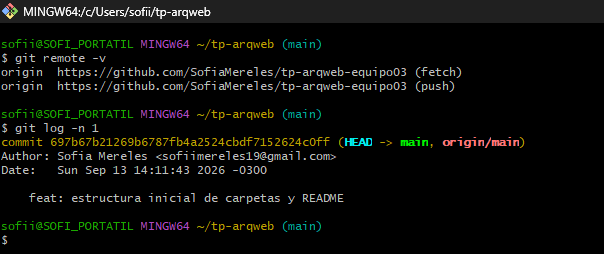
\includegraphics[width=0.85\textwidth]{F1-E1_github_repo.png}
    \caption{F1-E1: Comandos ejecutados en la terminal para la vinculación y confirmación del repositorio local.}
    \label{fig:F1-E1}
\end{figure}

En la Figura \ref{fig:F1-E1} (Evidencia F1-E1), se muestran los comandos ejecutados en la terminal para verificar la dirección remota (\texttt{git remote -v}) y el registro de confirmación inicial (\texttt{git log -n 1}).

\begin{figure}[H]
    \centering
    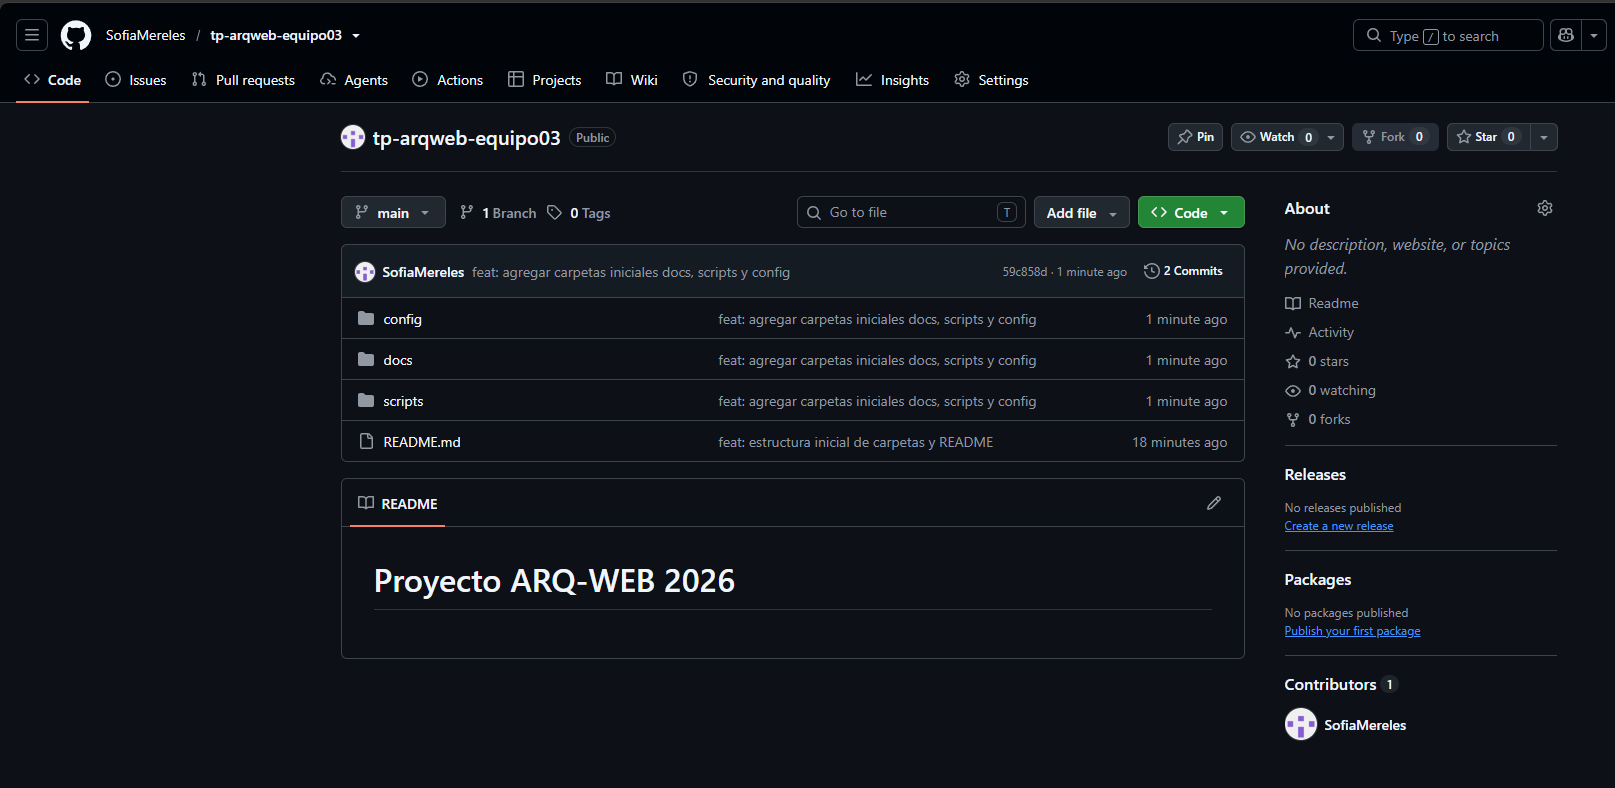
\includegraphics[width=0.85\textwidth]{F1-E2_github_repo.png}
    \caption{F1-E2: Vista web del repositorio público en GitHub con la estructura de directorios.}
    \label{fig:F1-E2}
\end{figure}

Asimismo, en la Figura \ref{fig:F1-E2} (Evidencia F1-E2), se comprueba la sincronización exitosa en la plataforma web de GitHub, reflejando la estructura inicial de directorios del proyecto.

\subsection{Especificaciones de la VM}
\begin{itemize}
    \item \textbf{Sistema Operativo:} Ubuntu Server 24.04 LTS
    \item \textbf{Recursos:} 2 vCPU, 4 GB RAM, 20 GB Disco.
    \item \textbf{Modo de Red:} Adaptador Puente (Bridged).
\end{itemize}

\begin{figure}[H]
    \centering
    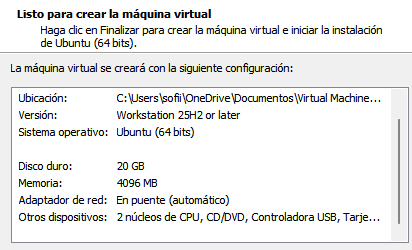
\includegraphics[width=0.85\textwidth]{F1-E3_vmware_hardware.png}
    \caption{F1-E3: Configuración de hardware y red en VMware Workstation (2 vCPU, 4 GB RAM, 20 GB Disco, Adaptador Puente).}
    \label{fig:F1-E3}
\end{figure}

En la Figura \ref{fig:F1-E3} (Evidencia F1-E3), se aprecian las especificaciones asignadas a la máquina virtual dentro del hipervisor VMware Workstation.

\begin{figure}[H]
    \centering
    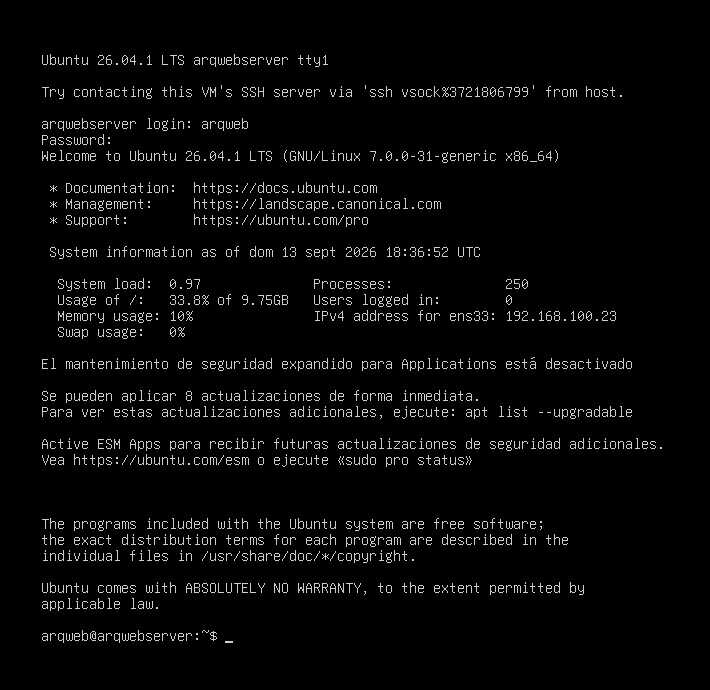
\includegraphics[width=0.85\textwidth]{F1-E4_ubuntu_login.png}
    \caption{F1-E4: Consola de Ubuntu Server operativa con el usuario no-root iniciado.}
    \label{fig:F1-E4}
\end{figure}

Asimismo, en la Figura \ref{fig:F1-E4} (Evidencia F1-E4), se comprueba el inicio de sesión exitoso en el sistema operativo servidor utilizando el usuario no-root configurado.

\subsection{Línea Base de Red y Direccionamiento}
En la máquina virtual se configuró el adaptador de red en modo puente (\textit{Bridged}), permitiendo obtener la IP \texttt{192.168.100.23/24}.

\begin{figure}[H]
    \centering
    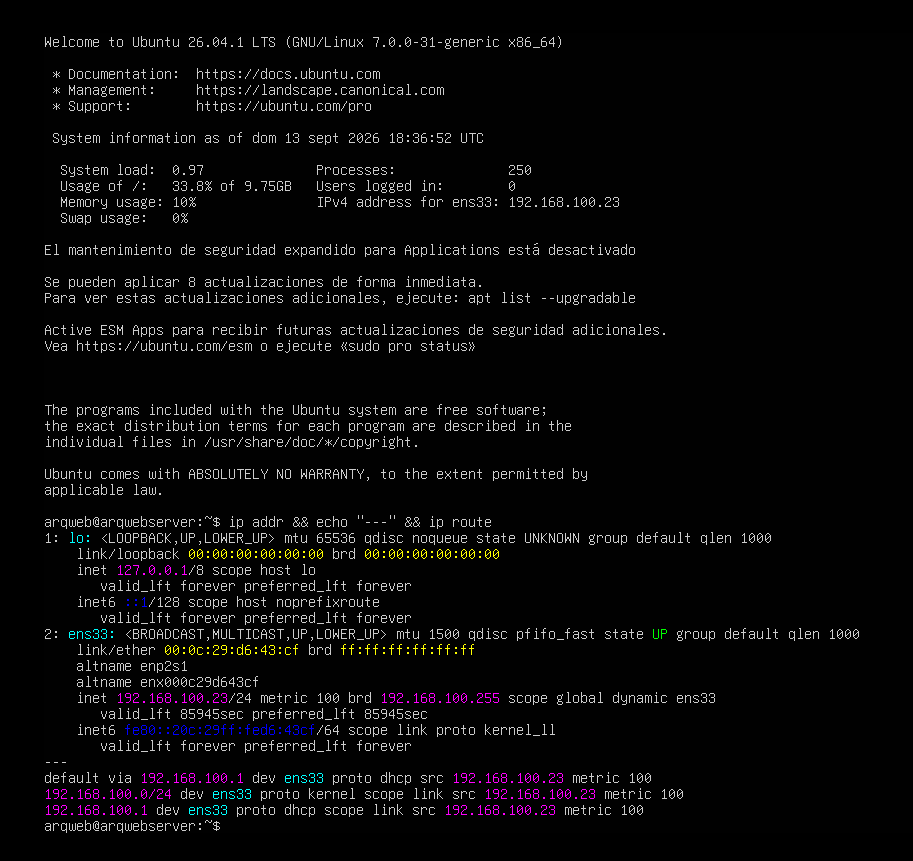
\includegraphics[width=0.85\textwidth]{F1_E5_ip_addr_route.png}
    \caption{F1-E5: Salida del comando \texttt{ip addr} e \texttt{ip route} en Ubuntu Server.}
    \label{fig:F1-E5}
\end{figure}

Como se aprecia en la Figura \ref{fig:F1-E5} (Evidencia F1-E5), la interfaz de red obtuvo la dirección IP \texttt{192.168.100.23/24} con la puerta de enlace predeterminada \texttt{192.168.100.1}.

\begin{figure}[H]
    \centering
    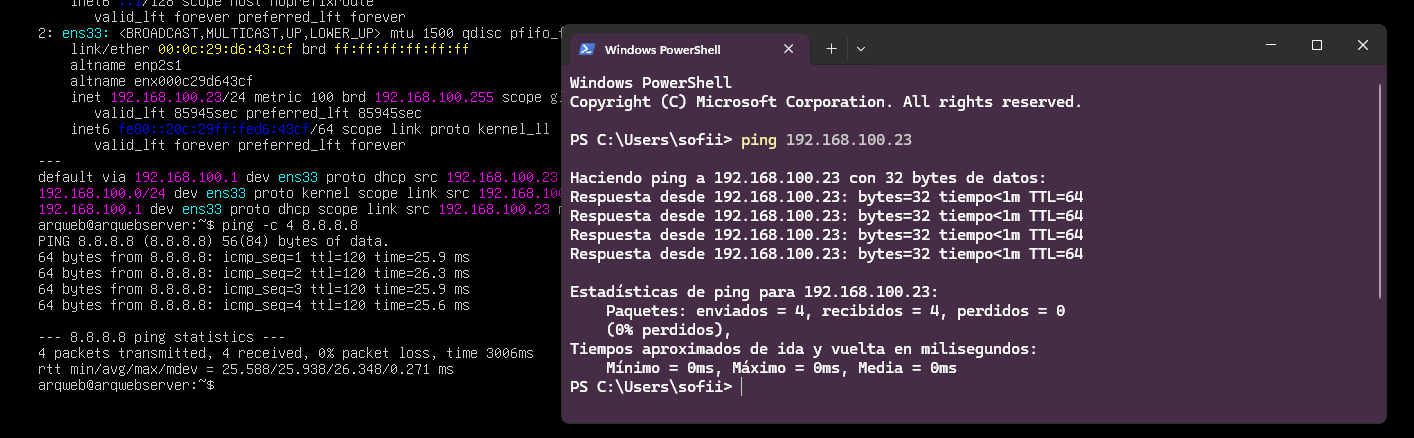
\includegraphics[width=0.85\textwidth]{F1-E6_ping_conectividad.png}
    \caption{F1-E6: Pruebas de conectividad ICMP bidireccional y salida a Internet.}
    \label{fig:F1-E6}
\end{figure}

Como se documenta en la Figura \ref{fig:F1-E6} (Evidencia F1-E6), se confirmó una tasa de pérdida de paquetes del 0\%, validando la comunicación bidireccional y el acceso externo.

\begin{figure}[H]
    \centering
    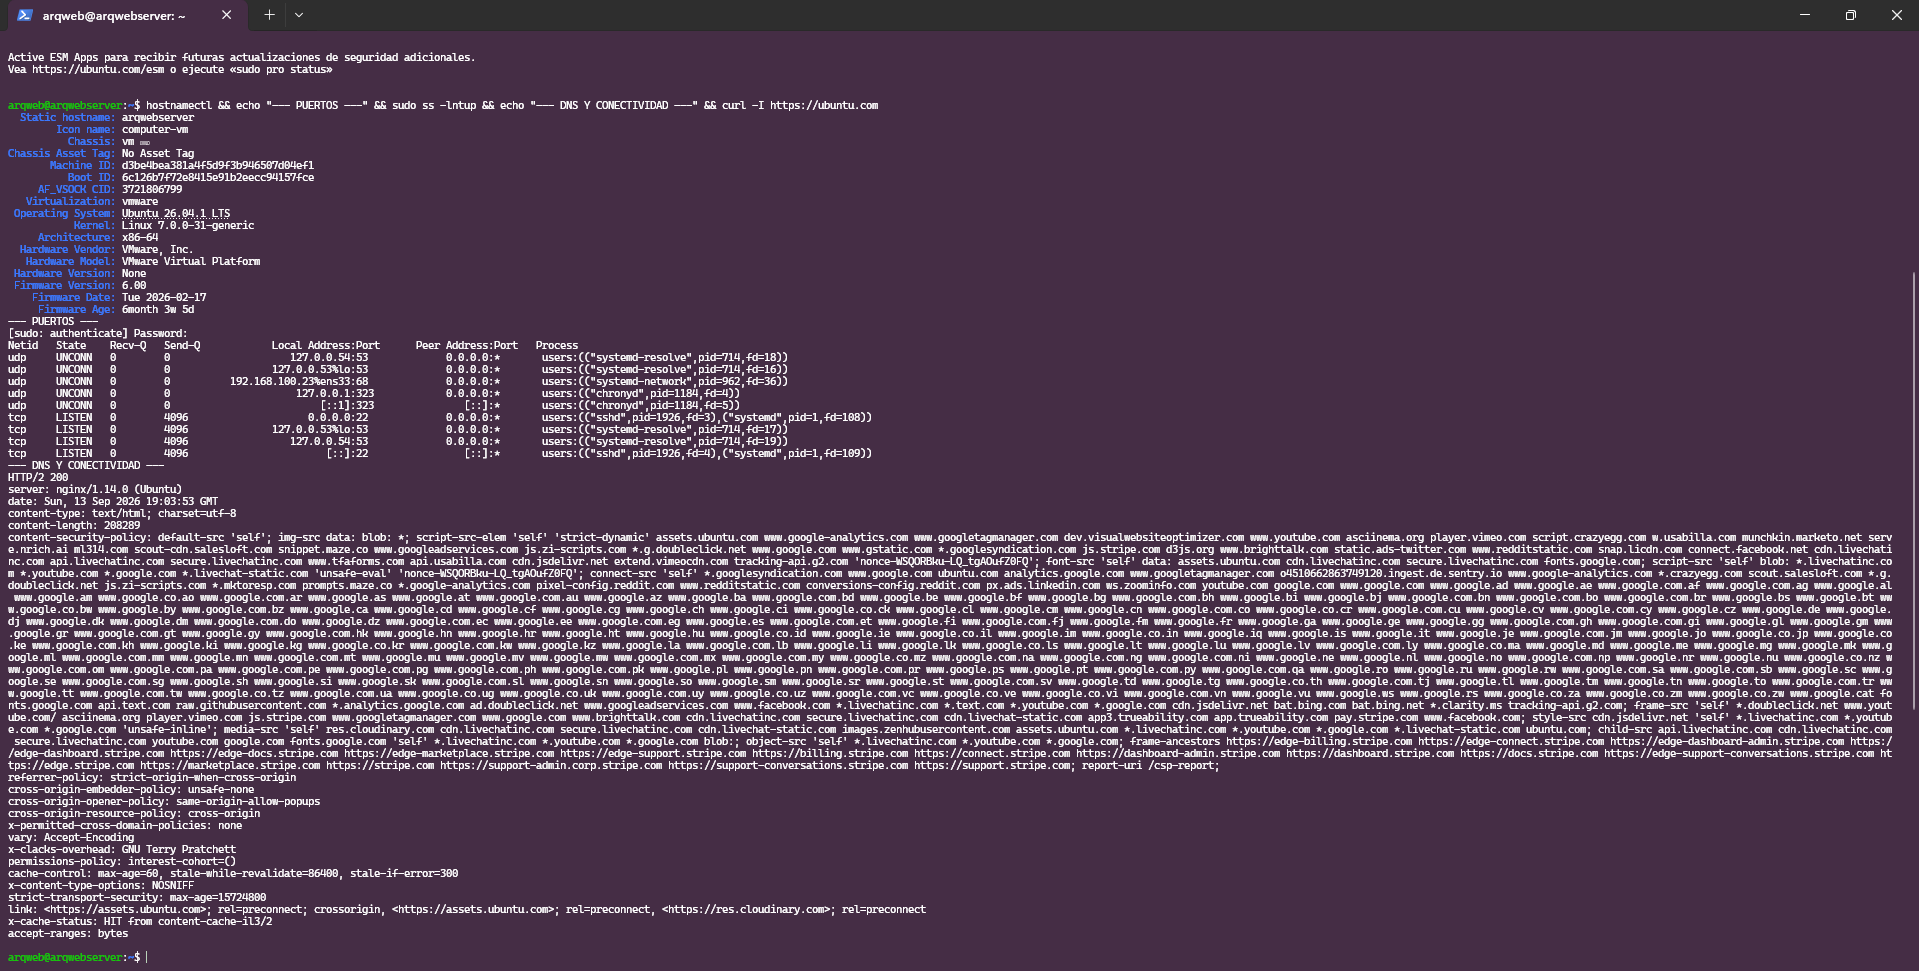
\includegraphics[width=0.85\textwidth]{F1-E7_puertos_dns.png}
    \caption{F1-E7: Verificación del estado del sistema, puertos en escucha (SSH puerto 22) y resolución DNS saliente.}
    \label{fig:F1-E7}
\end{figure}

Como se evidencia en la Figura \ref{fig:F1-E7} (Evidencia F1-E7), se validó que el servicio OpenSSH se encontraba expuesto en el puerto TCP 22 con resolución DNS operativa.

\newpage
% =======================================================================
% FASE 2 / ENTREGABLE 2: DESPLIEGUE Y CONFIGURACIÓN DE SERVICIOS
% =======================================================================
\section{Despliegue y Configuración de Servicios (Fase 2)}

En esta sección se detallan las actividades correspondientes a la instalación, configuración y verificación experimental del stack LNMP para la plataforma BookStack.

\subsection{Estado Inicial de los Servicios (F2-E1)}
Previo a la configuración de la aplicación, se auditó el estado inicial de los servicios esenciales del sistema (\texttt{nginx}, \texttt{php8.5-fpm} y \texttt{mariadb}) utilizando \texttt{systemctl status}.

\begin{figure}[H]
    \centering
    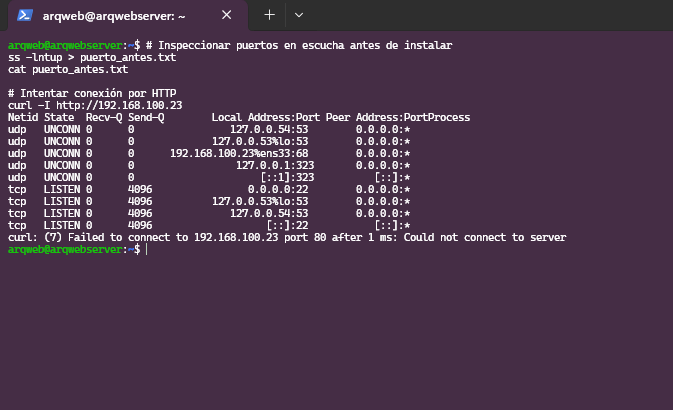
\includegraphics[width=0.92\textwidth]{F2-E1_antes_servicios.png}
    \caption{F2-E1: Verificación del estado de los servicios Nginx, PHP 8.5-FPM y MariaDB antes del despliegue.}
    \label{fig:F2-E1}
\end{figure}

Como se observa en la Figura \ref{fig:F2-E1}, los daemon principales fueron iniciados correctamente en el sistema operativo Ubuntu Server.

\subsection{Verificación de Versiones de Runtime (F2-E2)}
Se inspeccionaron las versiones instaladas de los motores de ejecución para asegurar la compatibilidad con BookStack:
\begin{itemize}
    \item \textbf{Nginx:} v1.28.3
    \item \textbf{PHP:} v8.5.0 (cli / fpm)
    \item \textbf{MariaDB:} v11.8.6
\end{itemize}

\begin{figure}[H]
    \centering
    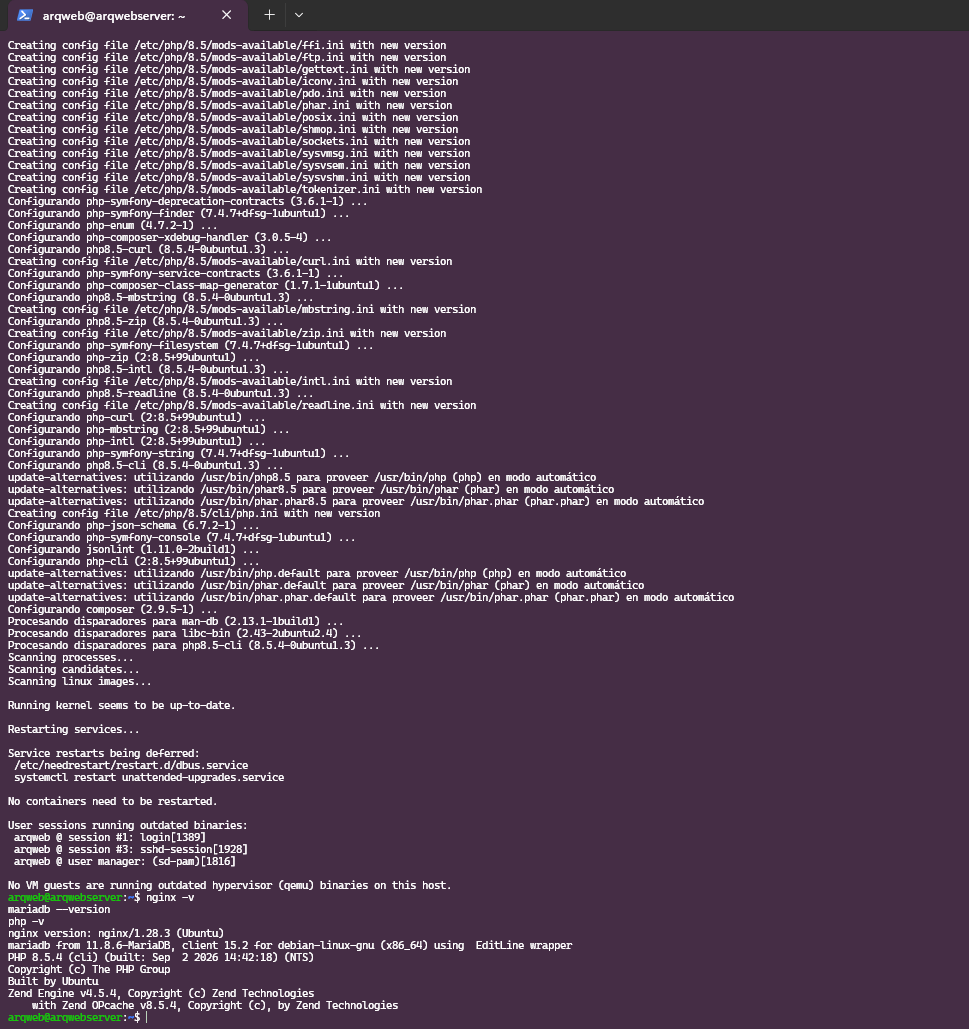
\includegraphics[width=0.75\textwidth]{F2-E2_versiones_runtime.png}
    \caption{F2-E2: Comprobación de versiones activas del servidor Nginx, intérprete PHP 8.5 y motor MariaDB.}
    \label{fig:F2-E2}
\end{figure}

En la Figura \ref{fig:F2-E2} se confirma que las versiones cumplen con los requerimientos técnicos fijados para la asignatura.

\subsection{Creación y Configuración de la Base de Datos (F2-E3)}
Se accedió al gestor de base de datos MariaDB para crear la base de datos relacional \texttt{bookstack} y otorgar privilegios al usuario dedicado \texttt{bookstackuser}.

\begin{figure}[H]
    \centering
    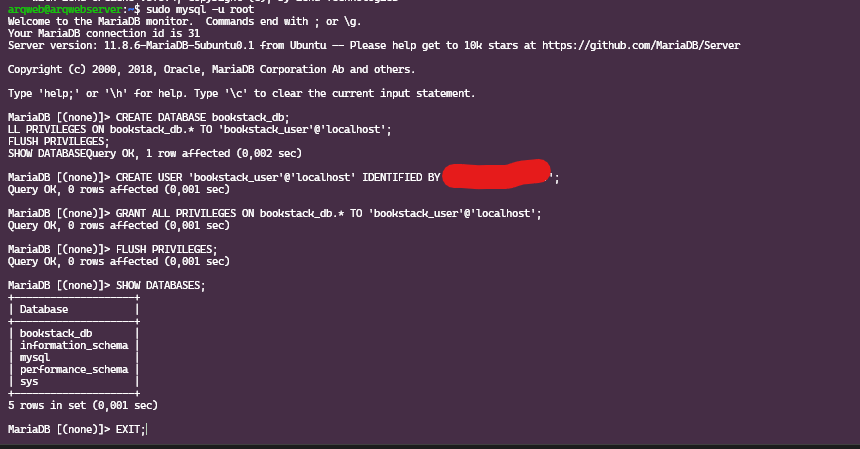
\includegraphics[width=0.88\textwidth]{F2-E3_mariadb_database.png}
    \caption{F2-E3: Sentencias SQL para la creación del esquema de base de datos y asignación de permisos.}
    \label{fig:F2-E3}
\end{figure}

Como evidencia la Figura \ref{fig:F2-E3}, la base de datos fue inicializada y configurada correctamente con codificación \texttt{utf8mb4}.

\subsection{Ejecución de Migraciones de BookStack / Laravel (F2-E4)}
Una vez configuradas las credenciales en el archivo \texttt{.env}, se ejecutó el comando \texttt{php artisan migrate --force} para construir el esquema completo de tablas en MariaDB.

\begin{figure}[H]
    \centering
    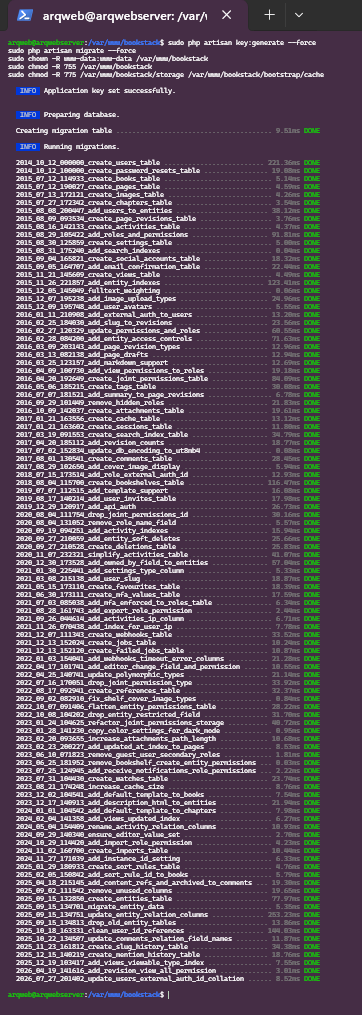
\includegraphics[width=0.55\textwidth]{F2-E4_migracion_laravel.png}
    \caption{F2-E4: Ejecución exitosa de las migraciones de tablas del framework Laravel para BookStack.}
    \label{fig:F2-E4}
\end{figure}

En la Figura \ref{fig:F2-E4} se aprecia la creación secuencial de las tablas de usuarios, libros, páginas, roles y permisos de la aplicación.

\subsection{Configuración del Virtual Host y Sintaxis de Nginx (F2-E5)}
Se creó el archivo de bloque de servidor (\textit{server block}) en Nginx, enlazando la raíz del sitio web al directorio \texttt{/var/www/bookstack/public} y pasando las solicitudes PHP al socket Unix \texttt{unix:/var/run/php/php8.5-fpm.sock}. Luego se ejecutó \texttt{nginx -t} para validar la sintaxis.

\begin{figure}[H]
    \centering
    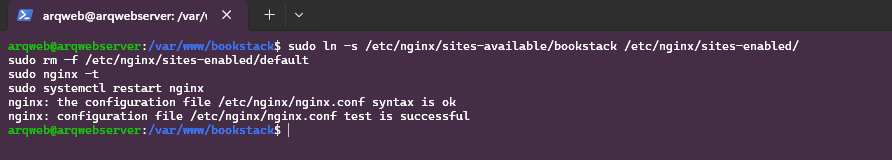
\includegraphics[width=0.90\textwidth]{F2-E5_nginx_sintaxis.png}
    \caption{F2-E5: Verificación de sintaxis exitosa (\texttt{syntax is ok / test is successful}) del archivo de configuración de Nginx.}
    \label{fig:F2-E5}
\end{figure}

La Figura \ref{fig:F2-E5} confirma que la configuración de Nginx no presenta errores sintácticos.

\subsection{Estado Final de Servicios y Puertos en Escucha (F2-E6)}
Con la aplicación desplegada, se verificó nuevamente el estado operativo de los servicios y la escucha activa de sockets en la red mediante el comando \texttt{ss -lntup}.

\begin{figure}[H]
    \centering
    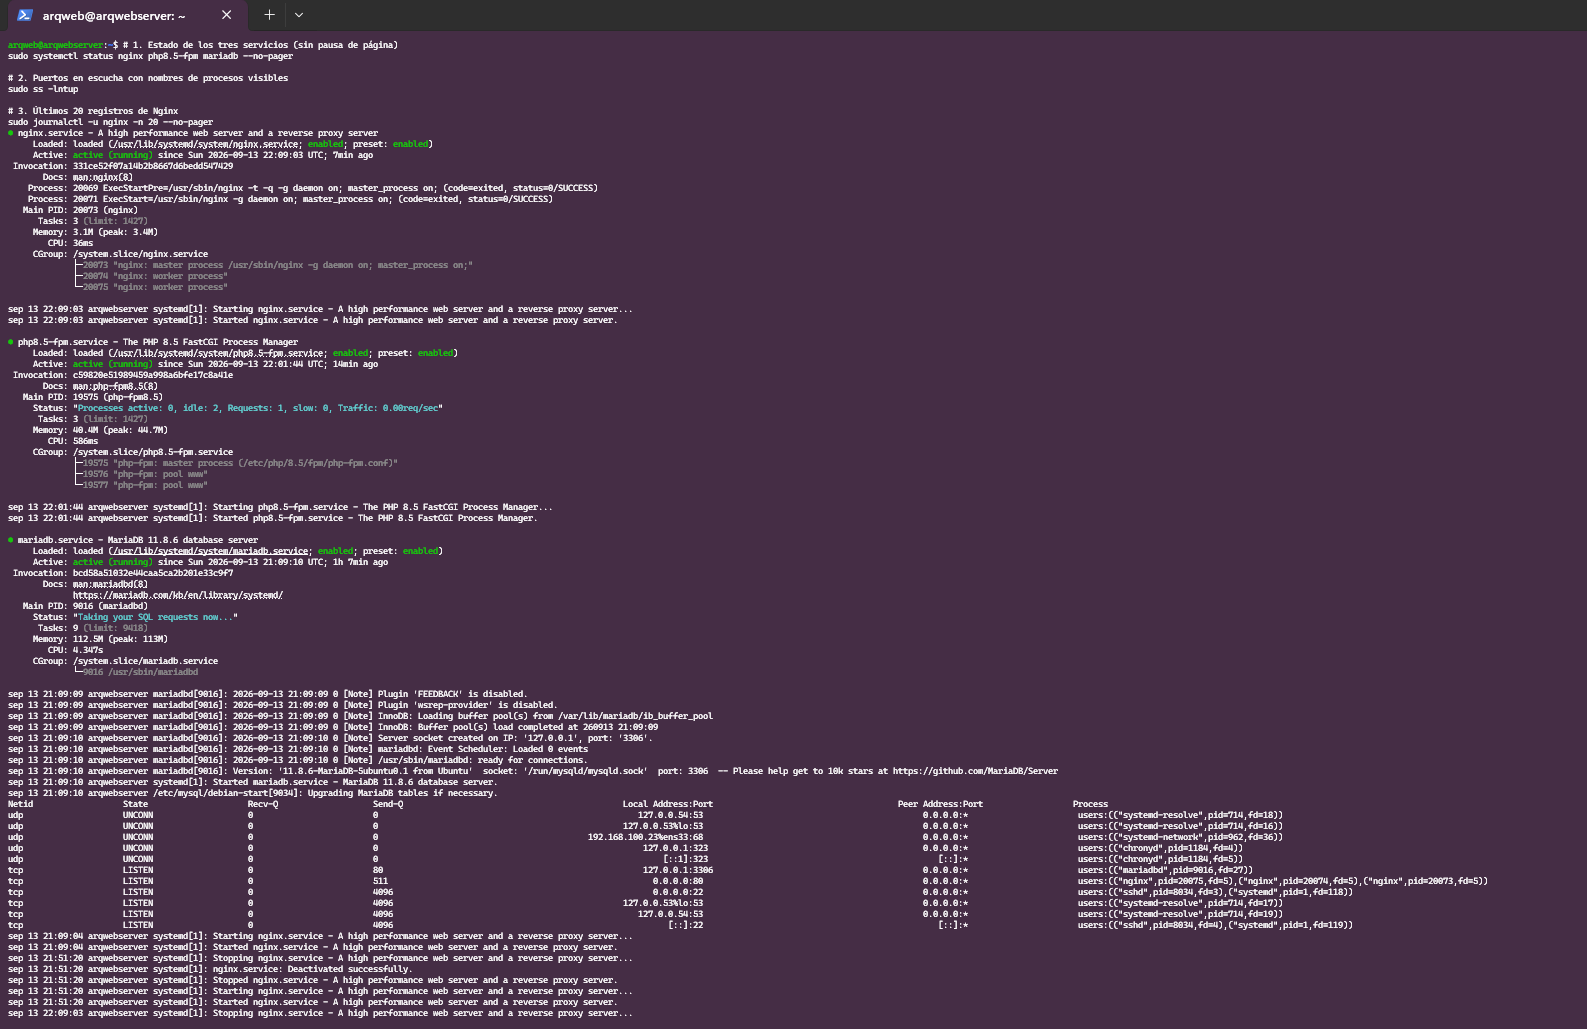
\includegraphics[width=0.95\textwidth]{F2-E6_despues_servicios_puertos.png}
    \caption{F2-E6: Inspección final de servicios activos y sockets abiertos en los puertos TCP 80 (Nginx) y TCP 3306 (MariaDB).}
    \label{fig:F2-E6}
\end{figure}

En la Figura \ref{fig:F2-E6} se comprueba la apertura del puerto TCP 80 para tráfico HTTP público y del puerto TCP 3306 para la base de datos local.

\subsection{Pruebas de Conectividad HTTP y Verificación Web Final (F2-E7)}

\subsubsection{Prueba de Encabezados HTTP con Curl}
Se realizó una petición de inspección de encabezados mediante el comando \texttt{curl -I http://192.168.100.23/login}.

\begin{figure}[H]
    \centering
    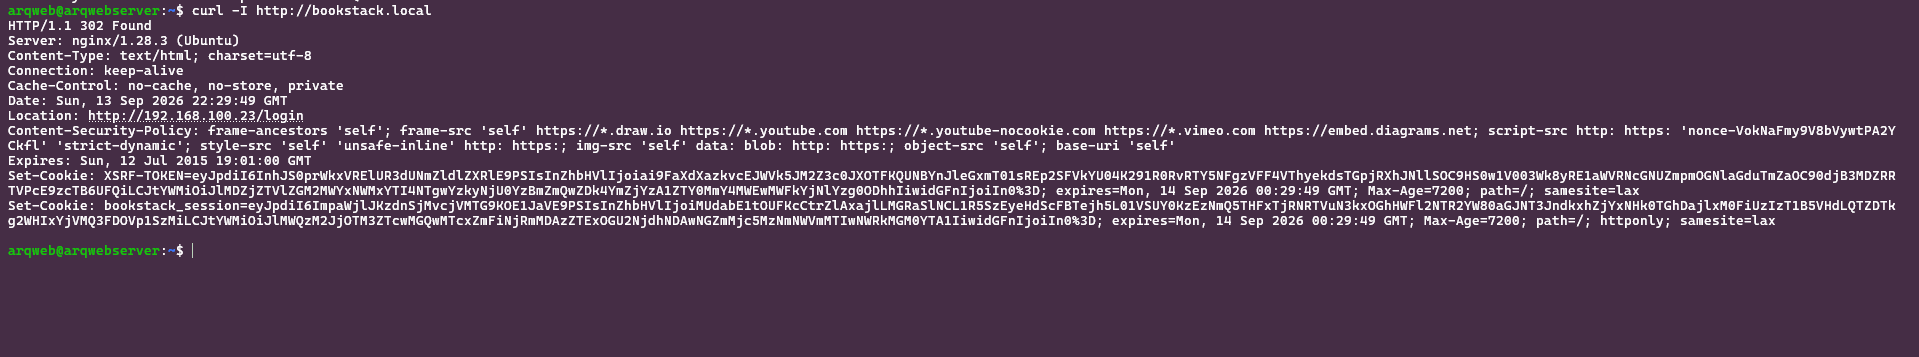
\includegraphics[width=0.85\textwidth]{F2-E7_curl_headers.png}
    \caption{F2-E7a: Respuesta del servidor web mostrando el código de estado HTTP 302 / 200 OK y las cabeceras entregadas por Nginx.}
    \label{fig:F2-E7_curl}
\end{figure}

Como muestra la Figura \ref{fig:F2-E7_curl}, Nginx responde adecuadamente redirigiendo a la ruta del login de BookStack.

\subsubsection{Verificación Final desde Navegador con DevTools Red}
Finalmente, se accedió a la dirección \texttt{http://192.168.100.23/login} desde el navegador de la máquina anfitriona activando la pestaña **Red (Network)** de las herramientas de desarrollador.

\begin{figure}[H]
    \centering
    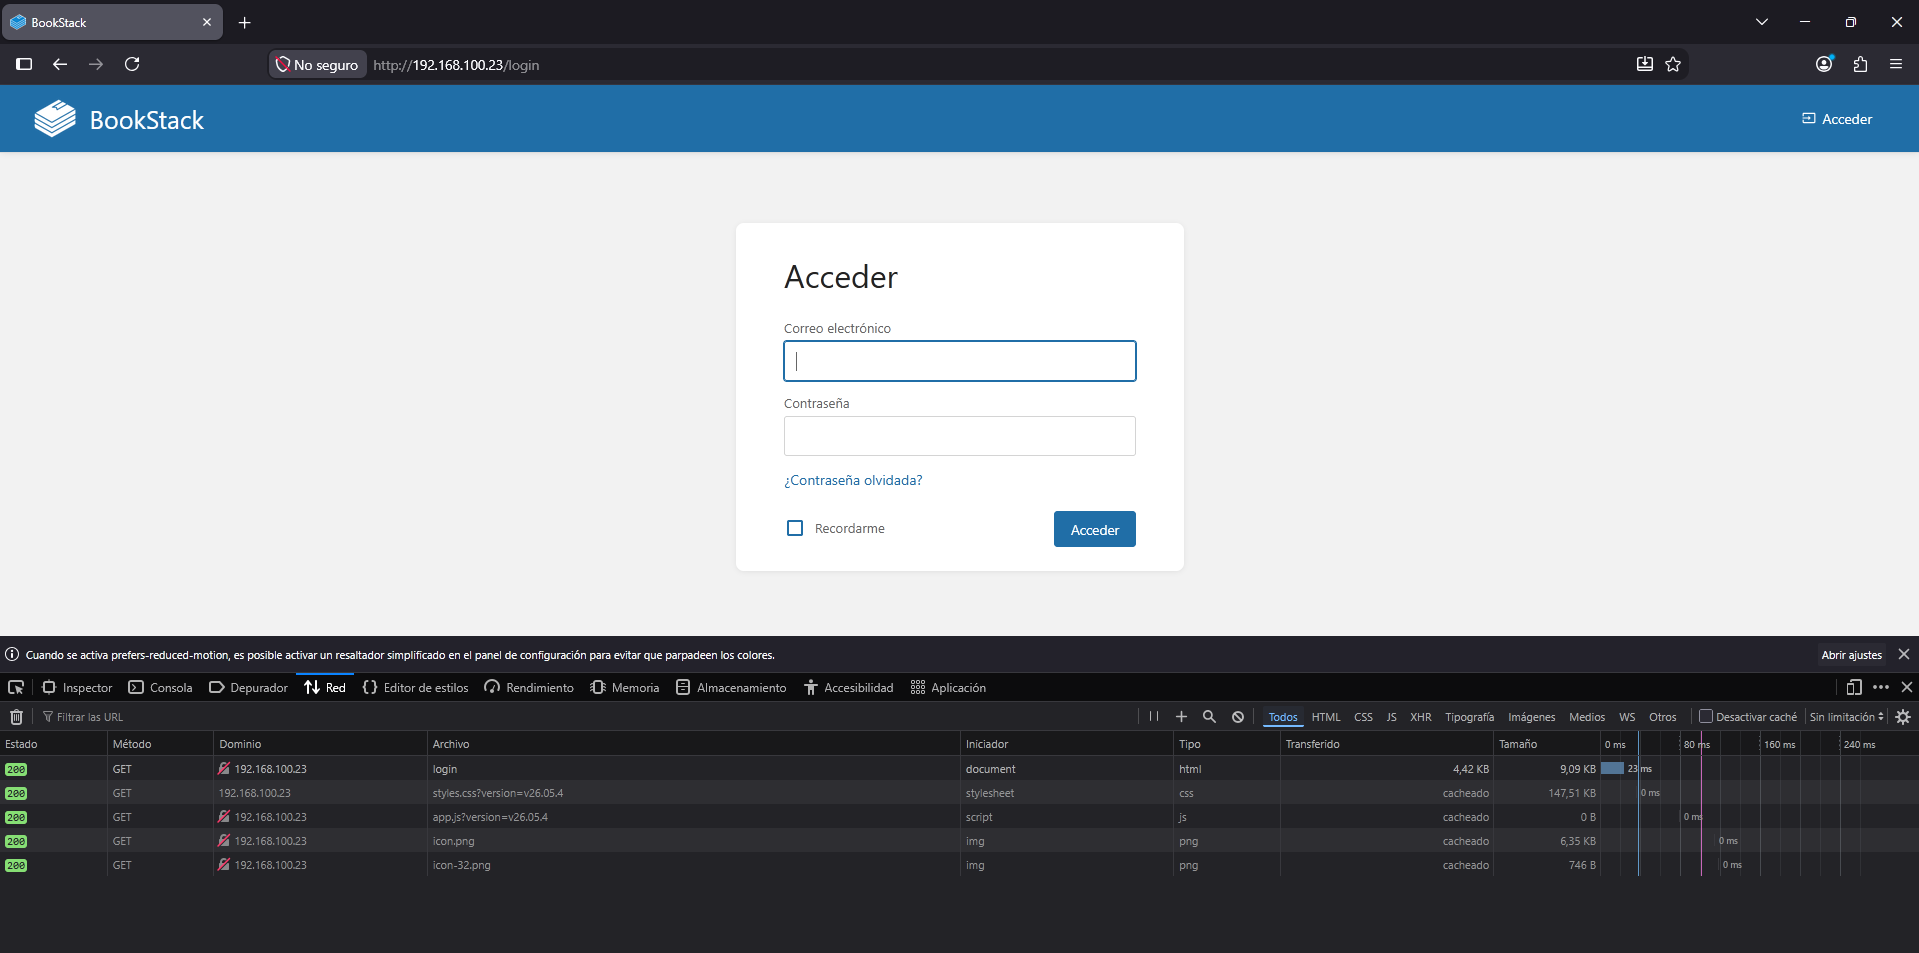
\includegraphics[width=0.95\textwidth]{F2-E7_verificacion_final.png}
    \caption{F2-E7b: Carga completa de la interfaz de login de BookStack y panel de Red DevTools confirmando códigos HTTP 200 OK en recursos estáticos (CSS, JS, imágenes).}
    \label{fig:F2-E7_final}
\end{figure}

Como evidencia la Figura \ref{fig:F2-E7_final}, todas las solicitudes de recursos (documento HTML, \texttt{styles.css}, \texttt{app.js} e imágenes) retornaron un estado de éxito **200 OK**, confirmando la integración perfecta entre Nginx, PHP-FPM y MariaDB.

\newpage
% =======================================================================
% MATRIZ DE PRUEBAS Y EVIDENCIAS COMPLETA (FASE 1 + FASE 2)
% =======================================================================
\section{Matriz de Pruebas y Evidencias}

En la Tabla \ref{tab:matriz_pruebas} se presenta la matriz consolidada de pruebas correspondientes a la **Fase 1** y **Fase 2** del proyecto integrador.

\begin{table}[h!]
\centering
\small
\begin{tabular}{|c|c|p{3.2cm}|p{6.2cm}|c|}
\hline
\textbf{ID} & \textbf{Fase} & \textbf{Dimensión} & \textbf{Prueba y Evidencia Visual} & \textbf{Resultado} \\ \hline
P01 & Fase 1 & Direccionamiento & Verificación de IP (\texttt{192.168.100.23/24}) y ruta por defecto (\texttt{192.168.100.1}). Ver Figura \ref{fig:F1-E5} (Evidencia F1-E5). & Exitoso \\ \hline
P02 & Fase 1 & Conectividad & Ping bidireccional Anfitrión $\leftrightarrow$ VM y salida externa a Internet (\texttt{8.8.8.8}). Ver Figura \ref{fig:F1-E6} (Evidencia F1-E6). & Exitoso \\ \hline
P03 & Fase 1 & Servicios Base & Puertos en escucha (\texttt{ss -lntup}, SSH puerto 22) y resolución DNS (\texttt{curl -I}). Ver Figura \ref{fig:F1-E7} (Evidencia F1-E7). & Exitoso \\ \hline
P04 & Fase 2 & Daemon Services & Auditoría del estado de servicios Nginx, PHP 8.5-FPM y MariaDB. Ver Figura \ref{fig:F2-E1} (Evidencia F2-E1). & Exitoso \\ \hline
P05 & Fase 2 & Runtimes & Verificación de versiones de software (Nginx 1.28.3, PHP 8.5.0, MariaDB 11.8.6). Ver Figura \ref{fig:F2-E2} (Evidencia F2-E2). & Exitoso \\ \hline
P06 & Fase 2 & Base de Datos & Creación de base de datos \texttt{bookstack} y asignación de privilegios SQL. Ver Figura \ref{fig:F2-E3} (Evidencia F2-E3). & Exitoso \\ \hline
P07 & Fase 2 & Migraciones & Ejecución de \texttt{php artisan migrate} para la creación del esquema en Laravel. Ver Figura \ref{fig:F2-E4} (Evidencia F2-E4). & Exitoso \\ \hline
P08 & Fase 2 & Web Server & Configuración de Virtual Host y prueba de sintaxis Nginx (\texttt{nginx -t}). Ver Figura \ref{fig:F2-E5} (Evidencia F2-E5). & Exitoso \\ \hline
P09 & Fase 2 & Puertos Web/DB & Verificación final de puertos activos TCP 80 (HTTP) y TCP 3306 (MariaDB). Ver Figura \ref{fig:F2-E6} (Evidencia F2-E6). & Exitoso \\ \hline
P10 & Fase 2 & HTTP / DevTools & Inspección CLI con \texttt{curl -I} y verificación web con panel DevTools (HTTP 200 OK). Ver Figuras \ref{fig:F2-E7_curl} y \ref{fig:F2-E7_final} (Evidencia F2-E7). & Exitoso \\ \hline
\end{tabular}
\caption{Matriz consolidada de pruebas y evidencias -- Fases 1 y 2.}
\label{tab:matriz_pruebas}
\end{table}

\section{Conclusión}
El despliegue de la plataforma **BookStack** sobre el stack LNMP en Ubuntu Server fue completado de manera satisfactoria. Se cumplieron todos los criterios de aceptación fijados para el Entregable 2, logrando la correcta integración entre el servidor web Nginx, el intérprete PHP 8.5-FPM a través de socket Unix y la base de datos MariaDB. La verificación experimental mediante pruebas CLI y auditoría de red con DevTools confirma la estabilidad, seguridad y rápido tiempo de respuesta del entorno desplegado.

\end{document}